\section{Results}
\label{sec:slam-results}
This section presents the empirical results from the evaluation of three localisation configurations: the baseline GLIM algorithm with default parameters, the refined GLIM algorithm with optimised parameters, and the proposed GNSS-augmented method. Each configuration was evaluated on five parameterisation datasets; additionally, all three configurations were evaluated on a held-out Evaluation Dataset, described in \cref{subsec:slam-experimental-setup}, to assess generalisation to an unseen route. Performance is reported using Root Mean Square Error (RMSE), Absolute Trajectory Error (ATE), Relative Pose Error (RPE), and, for the proposed method, the Global Alignment and Smoothness Profile (GASP) metric defined in the methodology.

\subsection{Baseline GLIM Performance}

\cref{tab:baseline_performance} reports the performance of the baseline GLIM algorithm across the five datasets. The error percentage per metre ranges from 1.253\% (Dataset~1) to 7.361\% (Dataset~2). The 3D RMSE ranges from 8.035\,m (Dataset~1) to 38.107\,m (Dataset~3), and the ATE ranges from 6.605\,m to 30.444\,m. The maximum single-point 3D error observed is 80.339\,m in Dataset~2.

\begin{table}[htbp]
\centering
\caption{Baseline GLIM performance over the five test datasets}
\label{tab:baseline_performance}
\begin{tabularx}{\textwidth}{lXXXXX}
\toprule
\textbf{Metrics} & \textbf{Dataset 0} & \textbf{Dataset 1} & \textbf{Dataset 2} & \textbf{Dataset 3} & \textbf{Dataset 4} \\ \midrule
RMSE\ x\ (m)\ & 20.776 & 7.253 & 4.097 & 4.747 & 3.598 \\
RMSE\ y\ (m)\ & 3.730 & 2.766 & 3.391 & 4.596 & 4.889 \\
RMSE\ z\ (m)\ & 15.107 & 1.747 & 35.970 & 36.908 & 25.879 \\
RMSE\ 3D\ (m)\ & 26.990 & 8.035 & 36.755 & 38.107 & 27.767 \\
ATE\ (m)\ & 19.877 & 6.605 & 25.921 & 30.444 & 25.331 \\
max\ error\ 3D\ (m)\ & 47.892 & 17.766 & 80.339 & 69.878 & 56.729 \\
error\ per\ meter\ (m)\ & 0.0340 & 0.0130 & 0.0740 & 0.0490 & 0.0420 \\
error\ percent\ per\ meter\ (\%)\ & 3.3580 & 1.2530 & 7.3610 & 4.8970 & 4.1910 \\
RPE\ 1m\ translation\ RMSE\ & 0.4697 & 0.2944 & 0.7632 & 1.0127 & 0.5356 \\
RPE\ 1m\ translation\ mean\ & 0.3100 & 0.1390 & 0.3210 & 0.3790 & 0.3170 \\
RPE\ 1m\ translation\ std\ & 0.4125 & 0.2602 & 0.6767 & 0.9384 & 0.4285 \\
RPE\ 1m\ translation\ max\ & 3.4500 & 2.8930 & 4.1800 & 15.7180 & 2.8810 \\
RPE\ 10m\ translation\ RMSE\ & 2.3790 & 1.5040 & 3.3400 & 3.3230 & 2.5920 \\
RPE\ 10m\ translation\ mean\ & 2.2680 & 1.1230 & 2.8110 & 3.0490 & 2.4040 \\
RPE\ 10m\ translation\ std\ & 0.7134 & 1.0076 & 1.8240 & 1.4120 & 0.9390 \\
RPE\ 10m\ translation\ max\ & 6.6530 & 7.9020 & 11.2070 & 16.2210 & 7.0210 \\ \bottomrule
\end{tabularx}
\end{table}

\subsection{Refined GLIM Performance}

\cref{tab:refined_performance} reports the results for the refined GLIM algorithm following parameter optimisation. The error percentage per metre ranges from 0.6081\% (Dataset~1) to 3.6150\% (Dataset~2). The 3D RMSE ranges from 3.4808\,m (Dataset~1) to 25.1789\,m (Dataset~2), and the ATE ranges from 3.2315\,m to 12.6781\,m.

\begin{table}[htbp]
\centering
\caption{Refined GLIM performance over the five datasets}
\label{tab:refined_performance}
\begin{tabularx}{\textwidth}{lXXXXX}
\toprule
\textbf{Metrics} & \textbf{Dataset 0} & \textbf{Dataset 1} & \textbf{Dataset 2} & \textbf{Dataset 3} & \textbf{Dataset 4} \\ \midrule
RMSE\ x\ (m)\ & 6.3487 & 2.5059 & 3.6146 & 3.5669 & 1.1221 \\
RMSE\ y\ (m)\ & 3.2186 & 2.3727 & 24.9149 & 3.4499 & 2.6844 \\
RMSE\ z\ (m)\ & 0.6987 & 0.4545 & 0.3994 & 1.0413 & 2.1387 \\
RMSE\ 3D\ (m)\ & 7.1522 & 3.4808 & 25.1789 & 5.0705 & 3.6110 \\
ATE\ (m)\ & 5.9190 & 3.2315 & 12.6781 & 4.6763 & 3.3144 \\
max\ error\ 3D\ (m)\ & 14.3770 & 5.5867 & 71.0506 & 13.0417 & 5.8597 \\
error\ per\ meter\ (m)\ & 0.0087 & 0.0061 & 0.0362 & 0.0075 & 0.0067 \\
error\ percent\ per\ meter\ (\%)\ & 0.8735 & 0.6081 & 3.6150 & 0.7499 & 0.6680 \\
RPE\ 1m\ translation\ RMSE\ & 0.3907 & 0.2609 & 0.5692 & 0.8317 & 0.3689 \\
RPE\ 1m\ translation\ mean\ & 0.1471 & 0.0899 & 0.3037 & 0.1133 & 0.1358 \\
RPE\ 1m\ translation\ std\ & 0.3619 & 0.2449 & 0.4814 & 0.8239 & 0.3430 \\
RPE\ 1m\ translation\ max\ & 3.1190 & 2.8235 & 2.3976 & 15.1426 & 2.7154 \\
RPE\ 10m\ translation\ RMSE\ & 1.2280 & 1.5267 & 4.6931 & 2.6912 & 1.4290 \\
RPE\ 10m\ translation\ mean\ & 0.7309 & 0.5967 & 2.6938 & 0.8912 & 0.5826 \\
RPE\ 10m\ translation\ std\ & 0.9868 & 1.4052 & 3.8430 & 2.5394 & 1.3048 \\
RPE\ 10m\ translation\ max\ & 5.7503 & 7.7271 & 10.7189 & 15.4780 & 6.6573 \\ \bottomrule
\end{tabularx}
\end{table}


\subsection{Proposed Method Performance}

\cref{tab:proposed_performance} reports the results for the proposed GNSS-augmented method. The error percentage per metre ranges from 0.0153\% (Dataset~4) to 0.0501\% (Dataset~2). The 3D RMSE ranges from 0.1097\,m (Dataset~0) to 0.2280\,m (Dataset~2), and the ATE ranges from 0.0811\,m to 0.1741\,m. The GASP metric, which combines drift rate and local pose smoothness, returned values between 0.0274 (Dataset~0) and 0.0679 (Dataset~2).

\begin{table}[htbp]
\centering
\caption{Proposed method performance over the 5 test datasets}
\label{tab:proposed_performance}
\begin{tabularx}{\textwidth}{lXXXXX}
\toprule
\textbf{Metrics} & \textbf{Dataset 0} & \textbf{Dataset 1} & \textbf{Dataset 2} & \textbf{Dataset 3} & \textbf{Dataset 4} \\ \midrule
RMSE\ x\ (m)\ & 0.0756 & 0.0528 & 0.0909 & 0.0528 & 0.0728 \\
RMSE\ y\ (m)\ & 0.0645 & 0.0906 & 0.2003 & 0.0906 & 0.0789 \\
RMSE\ z\ (m)\ & 0.0465 & 0.0347 & 0.0599 & 0.0347 & 0.0560 \\
RMSE\ 3D\ (m)\ & 0.1097 & 0.1105 & 0.2280 & 0.1105 & 0.1211 \\
ATE\ (m)\ & 0.0846 & 0.0811 & 0.1741 & 0.0811 & 0.1031 \\
max\ error\ 3D\ (m)\ & 0.7363 & 0.8963 & 1.0246 & 0.8963 & 0.7056 \\
error\ per\ meter\ (m)\ & 0.0002 & 0.0002 & 0.0005 & 0.0002 & 0.0002 \\
error\ percent\ per\ meter\ (\%)\ & 0.0171 & 0.0154 & 0.0501 & 0.0154 & 0.0153 \\
gasp & 0.0274 & 0.0290 & 0.0679 & 0.0290 & 0.0429 \\
RPE\ 1m\ translation\ RMSE\ & 0.0270 & 0.0308 & 0.0556 & 0.0308 & 0.0444 \\
RPE\ 1m\ translation\ mean\ & 0.0175 & 0.0206 & 0.0282 & 0.0206 & 0.0249 \\
RPE\ 1m\ translation\ std\ & 0.0205 & 0.0229 & 0.0479 & 0.0229 & 0.0368 \\
RPE\ 1m\ translation\ max\ & 0.2001 & 0.4906 & 0.6992 & 0.4906 & 0.6462 \\
RPE\ 10m\ translation\ RMSE\ & 0.0649 & 0.0936 & 0.1772 & 0.0936 & 0.0769 \\
RPE\ 10m\ translation\ mean\ & 0.0433 & 0.0613 & 0.0987 & 0.0613 & 0.0573 \\
RPE\ 10m\ translation\ std\ & 0.0482 & 0.0708 & 0.1471 & 0.0708 & 0.0512 \\
RPE\ 10m\ translation\ max\ & 0.3799 & 0.7620 & 0.8566 & 0.7620 & 0.5377 \\ \bottomrule
\end{tabularx}
\end{table}

\subsection{Comparative Summary}

\cref{tab:comparison_table_key_metrics} presents a side-by-side comparison of the three methods on three key metrics: error percentage per metre, RPE 1\,m translation standard deviation, and error per metre. The lowest value for each metric--dataset combination is indicated in bold.

\begin{table}[htbp]
\centering
\caption{Comparison Table of the Key Metrics (Best results in bold)}
\label{tab:comparison_table_key_metrics}
\begin{tabularx}{\textwidth}{>{\hsize=0.8\hsize}X >{\hsize=1.2\hsize}X XXXXX} % Adjusting relative widths
\toprule
\textbf{Metric} & \textbf{Method} & \textbf{Dataset 0} & \textbf{Dataset 1} & \textbf{Dataset 2} & \textbf{Dataset 3} & \textbf{Dataset 4} \\ \midrule

% Use {=} in multirow to allow text wrapping inside the X column
\multirow{3}{=}{error percent per meter (\%)} & Baseline GLIM & 3.3580 & 1.2530 & 7.3610 & 4.8970 & 4.1910 \\
 & Refined GLIM & 0.8735 & 0.6081 & 3.6150 & 0.7499 & 0.6680 \\
 & Proposed Method & \textbf{0.0171} & \textbf{0.0154} & \textbf{0.0501} & \textbf{0.0154} & \textbf{0.0153} \\ \midrule

\multirow{3}{=}{RPE 1m translation std} & Baseline GLIM & 0.4125 & 0.2602 & 0.6767 & 0.9384 & 0.4285 \\
 & Refined GLIM & 0.3619 & 0.2449 & 0.4814 & 0.8239 & 0.3430 \\
 & Proposed Method & \textbf{0.0205} & \textbf{0.0229} & \textbf{0.0479} & \textbf{0.0229} & \textbf{0.0368} \\ \midrule

\multirow{3}{=}{error per meter (m)} & Baseline GLIM & 0.0340 & 0.0130 & 0.0740 & 0.0490 & 0.0420 \\
 & Refined GLIM & 0.0087 & 0.0061 & 0.0362 & 0.0075 & 0.0067 \\
 & Proposed Method & \textbf{0.0002} & \textbf{0.0002} & \textbf{0.0005} & \textbf{0.0002} & \textbf{0.0002} \\ \bottomrule
\end{tabularx}
\end{table}

\subsection{GNSS Factor Utilisation}

\cref{tab:gnss_stats} reports the number of GNSS factors incorporated into the proposed method's factor graph relative to the total number of available GNSS measurements. Across the five datasets, the proportion of GNSS points retained after outlier rejection and incorporated as factors ranges from 0.65\% (Dataset~2) to 0.78\% (Dataset~3).

\begin{table}[htbp]
\centering
\caption{Statistics on the number of GNSS factors used for the proposed method}
\label{tab:gnss_stats}
\begin{tabularx}{\textwidth}{lXXXXX}
\toprule
\textbf{Metric} & \textbf{Dataset 0} & \textbf{Dataset 1} & \textbf{Dataset 2} & \textbf{Dataset 3} & \textbf{Dataset 4} \\ \midrule
Number of factors & 93 & 73 & 47 & 86 & 69 \\
Number of GNSS points & 13461 & 10090 & 7236 & 11071 & 9241 \\
Percent of GNSS points used & 0.69 & 0.72 & 0.65 & 0.78 & 0.75 \\ \bottomrule
\end{tabularx}
\end{table}

\subsection{Parameter Optimisation Progression}

\cref{fig:comparison_dist} shows the distribution of per-iteration errors across the four optimisation stages. \cref{fig:baseline_error_dist} plots the error percentage per metre for the baseline GLIM tuning, and \cref{fig:proposed_error_dist} plots the GASP metric for the proposed method tuning. Both plots use a logarithmic horizontal axis.

\begin{figure}[htbp]
     \centering
     % Increased width to 0.8 to make them larger now that they are stacked
     \begin{subfigure}[b]{0.8\textwidth}
         \centering
         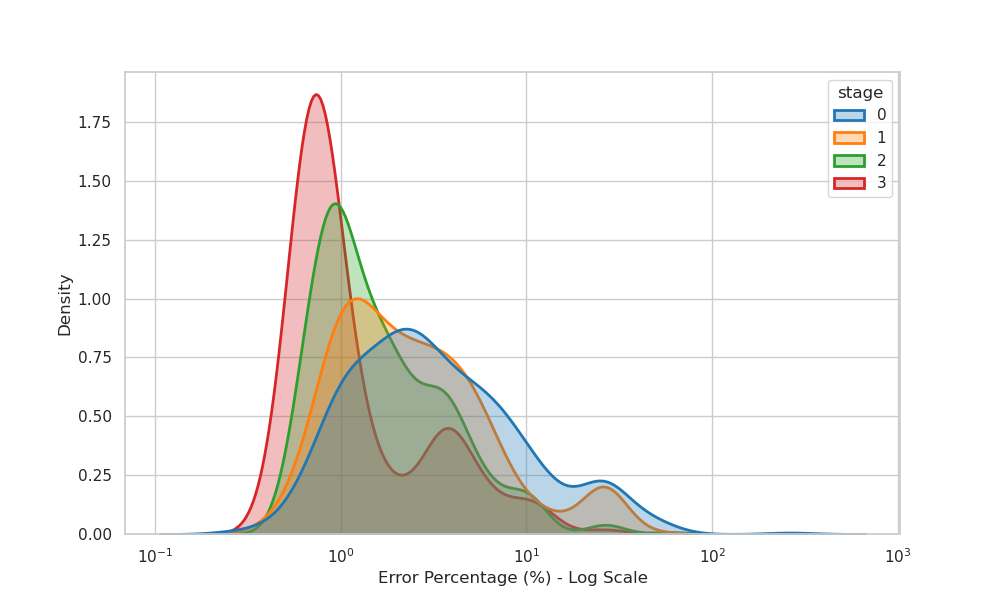
\includegraphics[width=\textwidth]{3-SLAM/3-results/figures/glim_error_distribution_by_stage_log.png}
         \caption{Baseline glim tuning.}
         \label{fig:baseline_error_dist}
     \end{subfigure}
     
     \vspace{1em} % Adds a little vertical space between the two images
     
     \begin{subfigure}[b]{0.8\textwidth}
         \centering
         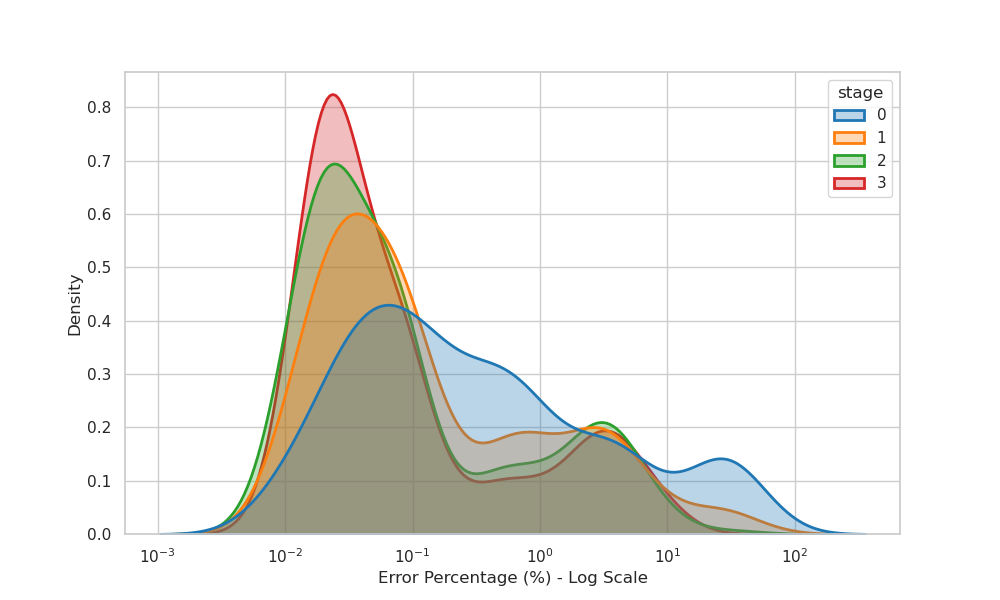
\includegraphics[width=\textwidth]{3-SLAM/3-results/figures/proposed_error_distribution_by_stage_log.png}
         \caption{Proposed method tuning.}
         \label{fig:proposed_error_dist}
     \end{subfigure}
     
     \caption{Error distribution (log scale) over optimisation stages for baseline tuning (error = error percentage) and proposed method tuning (error = GASP).}
     \label{fig:comparison_dist}
\end{figure}

\cref{fig:comparison_progression} plots the best consensus error at the end of each optimisation stage. \cref{fig:baseline_progression} tracks the error percentage for the baseline GLIM, and \cref{fig:proposed_progression} tracks the GASP metric for the proposed method. The baseline error decreases monotonically across the four stages; the proposed method's GASP score increases from stage~0 to stage~3.

\begin{figure}[htbp]
     \centering
     % Increased width from 0.48 to 0.8 for better visibility
     \begin{subfigure}[b]{0.8\textwidth}
         \centering
         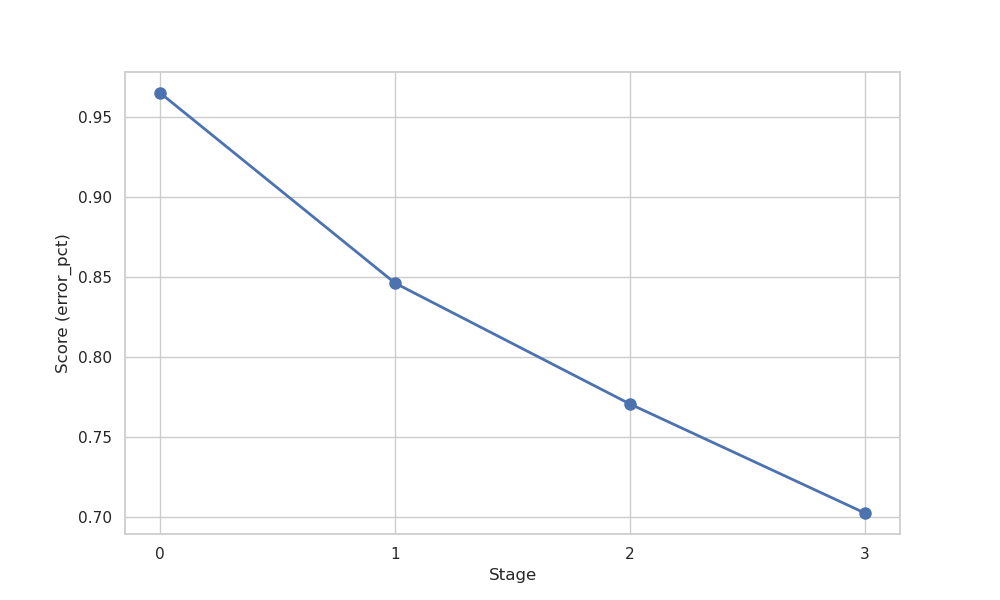
\includegraphics[width=\textwidth]{3-SLAM/3-results/figures/glim_consensus_progression.png}
         \caption{Baseline GLIM error percentage.}
         \label{fig:baseline_progression}
     \end{subfigure}

     \vspace{1.5em} % Adds vertical breathing room between the two plots

     \begin{subfigure}[b]{0.8\textwidth}
         \centering
         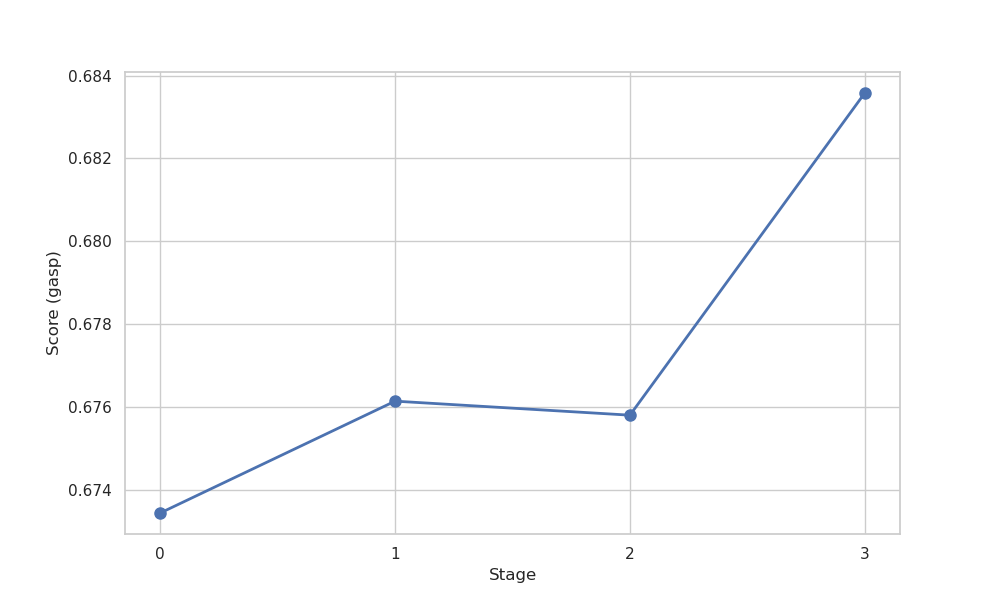
\includegraphics[width=\textwidth]{3-SLAM/3-results/figures/proposed_consensus_progression.png}
         \caption{Proposed Method GASP error.}
         \label{fig:proposed_progression}
     \end{subfigure}
     
     \caption{Consensus error over optimisation stages for baseline tuning (error = error percentage) and proposed method tuning (error = GASP).}
     \label{fig:comparison_progression}
\end{figure}

\subsection{Multi-Metric Radar Comparison}

\cref{fig:comparison_spider} presents four radar plots comparing the baseline, refined, and proposed methods across all five datasets. The four metrics displayed are error per metre, error percentage per metre, ATE, and RPE 1\,m translation standard deviation. Radial axes are plotted on a logarithmic scale.

\begin{figure}[htbp]
     \centering
     \begin{subfigure}[b]{0.48\textwidth}
         \centering
         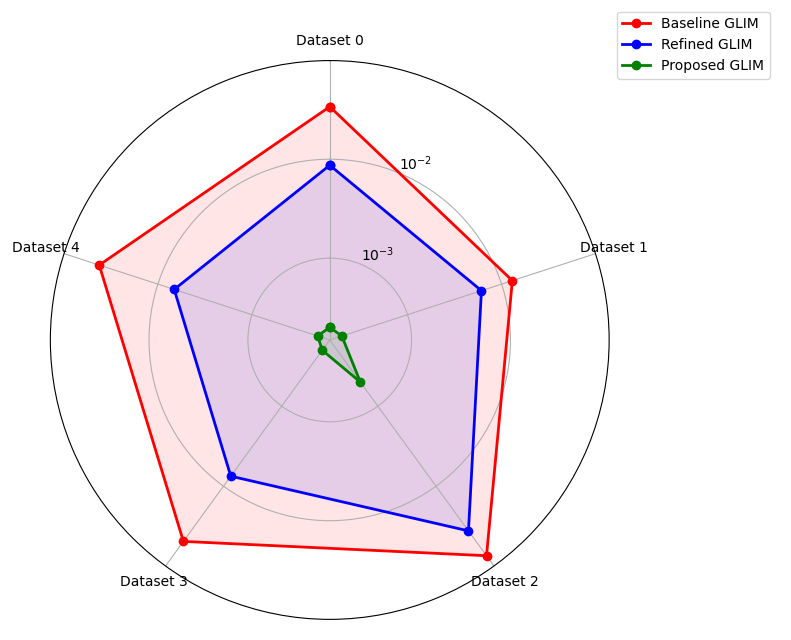
\includegraphics[width=\textwidth]{3-SLAM/3-results/figures/spider_error_per_m.png}
         \caption{Error per meter (m)}
         \label{fig:spider_epm}
     \end{subfigure}
     \hfill
     \begin{subfigure}[b]{0.48\textwidth}
         \centering
         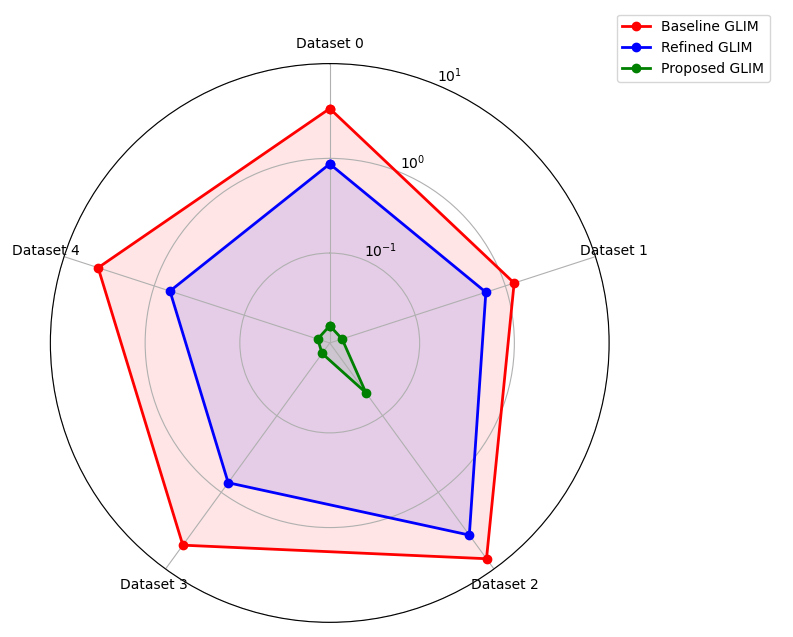
\includegraphics[width=\textwidth]{3-SLAM/3-results/figures/spider_error_pct.png}
         \caption{Error percent per meter.}
         \label{fig:spider_ep}
     \end{subfigure}
     \hfill
     \begin{subfigure}[b]{0.48\textwidth}
         \centering
         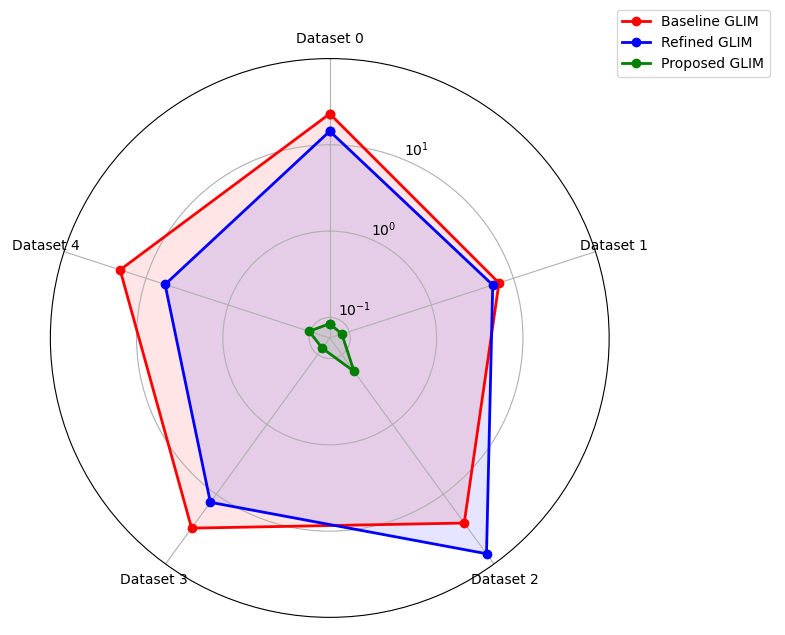
\includegraphics[width=\textwidth]{3-SLAM/3-results/figures/spider_mean_abs_pos_err.png}
         \caption{ATE error (m).}
         \label{fig:spider_ATE}
     \end{subfigure}
     \hfill
     \begin{subfigure}[b]{0.48\textwidth}
         \centering
         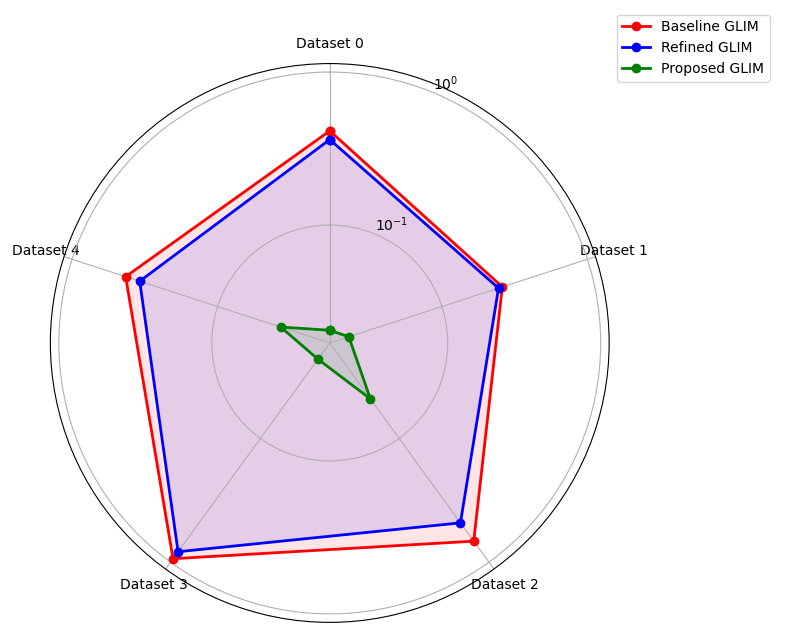
\includegraphics[width=\textwidth]{3-SLAM/3-results/figures/spider_rpe_1m_trans_std.png}
         \caption{RPE (translation only) standard deviation.} 
         \label{fig:spider_RPE_std}
     \end{subfigure}
     \caption{Spider plot comparisons of the glim baseline, refined and proposed methods for various key performance metrics.}
     \label{fig:comparison_spider}
\end{figure}

\subsection{Trajectory Visualisation}

\cref{fig:large_grid_xy} presents the planar ($x$--$y$) trajectories for each dataset. The left column shows the refined GLIM output and the right column shows the proposed method output, both plotted against the RTK~GNSS ground truth.

\begin{figure}[htbp]
    \centering
    % --- ROW 1 ---
    \begin{subfigure}[b]{0.48\textwidth}
        \centering
        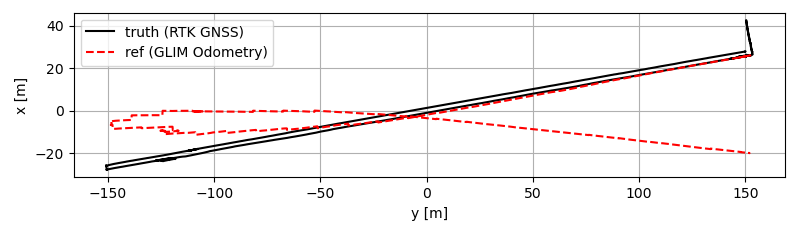
\includegraphics[width=\textwidth]{3-SLAM/3-results/figures/ds0_xy.png}
        \caption{Baseline | Dataset 0}
    \end{subfigure}
    \hfill
    \begin{subfigure}[b]{0.48\textwidth}
        \centering
        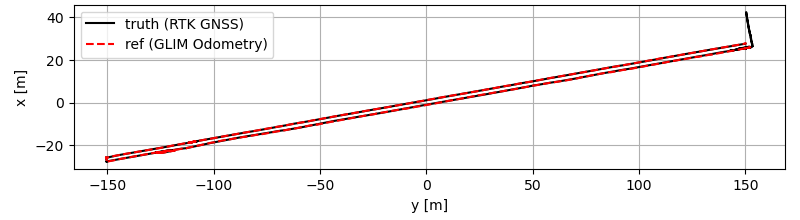
\includegraphics[width=\textwidth]{3-SLAM/3-results/figures/pds0_xy.png}
        \caption{Proposed | Dataset 0}
    \end{subfigure}

    \vspace{1em} % Vertical space between rows

    % --- ROW 2 ---
    \begin{subfigure}[b]{0.48\textwidth}
        \centering
        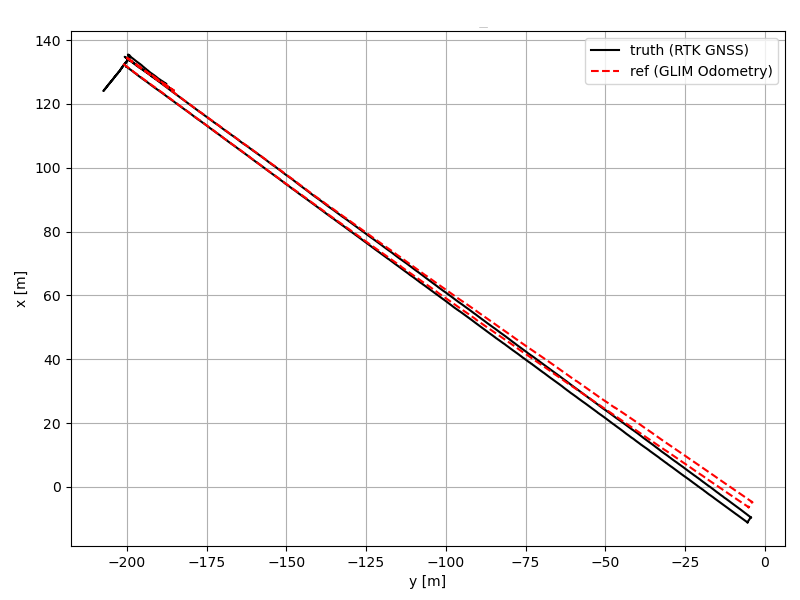
\includegraphics[width=\textwidth]{3-SLAM/3-results/figures/ds1_xy.png}
        \caption{Baseline | Dataset 1}
    \end{subfigure}
    \hfill
    \begin{subfigure}[b]{0.48\textwidth}
        \centering
        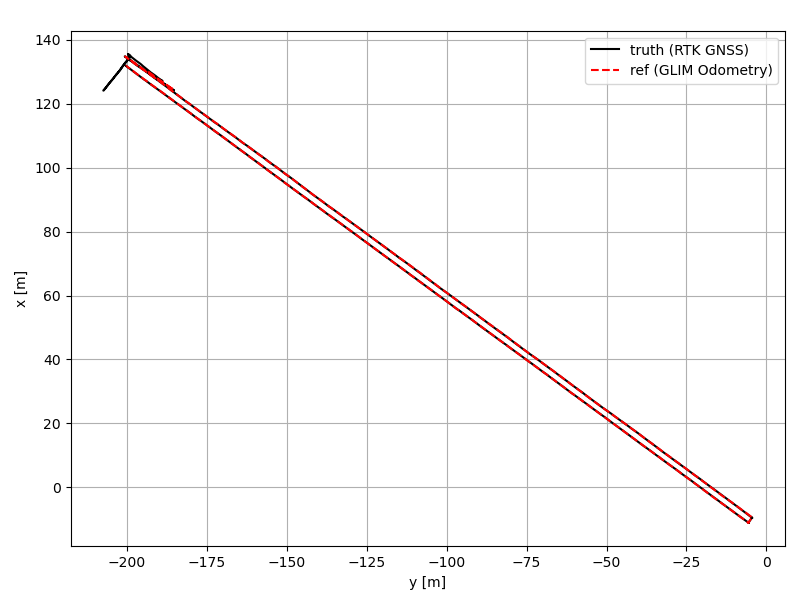
\includegraphics[width=\textwidth]{3-SLAM/3-results/figures/pds1_xy.png}
        \caption{Proposed | Dataset 1}
    \end{subfigure}

    \vspace{1em}

    % --- ROW 3 ---
    \begin{subfigure}[b]{0.48\textwidth}
        \centering
        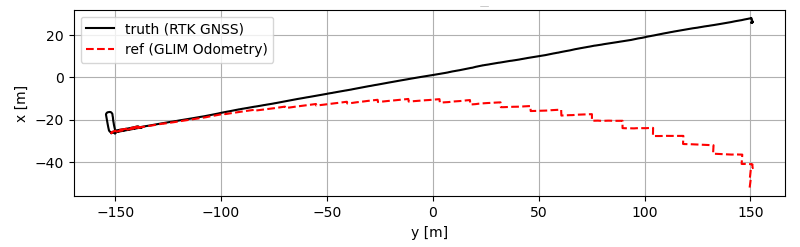
\includegraphics[width=\textwidth]{3-SLAM/3-results/figures/ds2_xy.png}
        \caption{Baseline | Dataset 2}
    \end{subfigure}
    \hfill
    \begin{subfigure}[b]{0.48\textwidth}
        \centering
        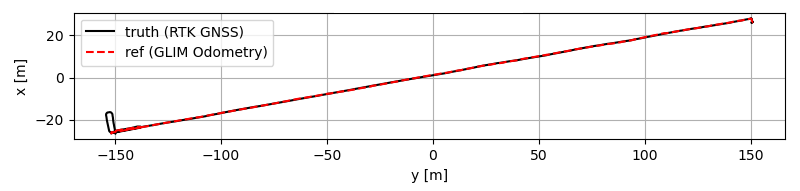
\includegraphics[width=\textwidth]{3-SLAM/3-results/figures/pds2_xy.png}
        \caption{Proposed | Dataset 2}
    \end{subfigure}

    \vspace{1em}

    % --- ROW 4 ---
    \begin{subfigure}[b]{0.48\textwidth}
        \centering
        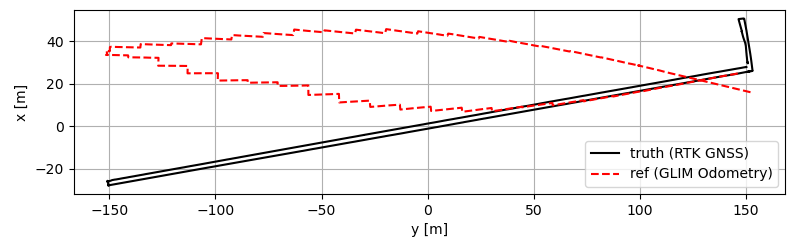
\includegraphics[width=\textwidth]{3-SLAM/3-results/figures/ds3_xy.png}
        \caption{Baseline | Dataset 3}
    \end{subfigure}
    \hfill
    \begin{subfigure}[b]{0.48\textwidth}
        \centering
        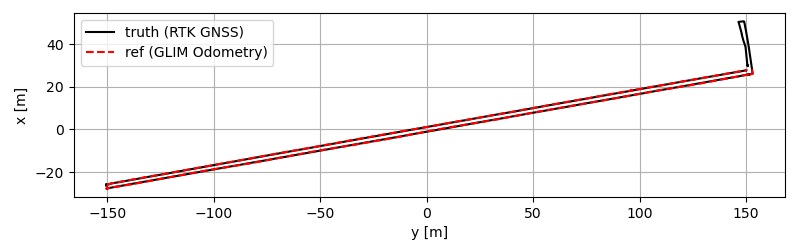
\includegraphics[width=\textwidth]{3-SLAM/3-results/figures/pds3_xy.png}
        \caption{Proposed | Dataset 3}
    \end{subfigure}

    \vspace{1em}

    % --- ROW 5 ---
    \begin{subfigure}[b]{0.48\textwidth}
        \centering
        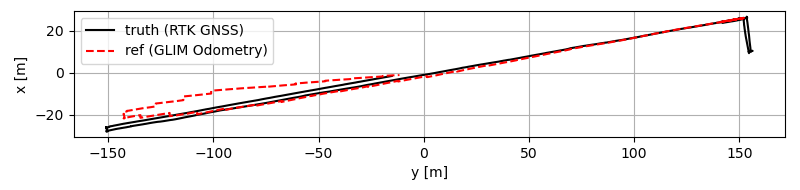
\includegraphics[width=\textwidth]{3-SLAM/3-results/figures/ds4_xy.png}
        \caption{Baseline | Dataset 4}
    \end{subfigure}
    \hfill
    \begin{subfigure}[b]{0.48\textwidth}
        \centering
        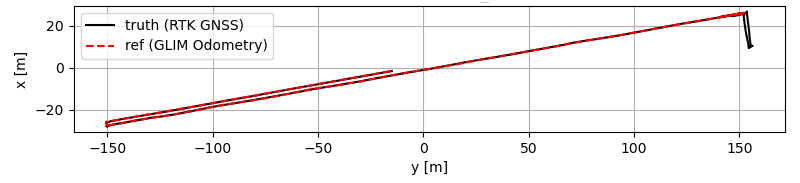
\includegraphics[width=\textwidth]{3-SLAM/3-results/figures/pds4_xy.png}
        \caption{Proposed | Dataset 4}
    \end{subfigure}

    \caption{Trajectories in XY plane from baseline GLIM and the proposed method.}
    \label{fig:large_grid_xy}
\end{figure}

\cref{fig:large_grid_z} presents the altitude ($z$-axis) trajectories for each dataset in the same layout, with the refined GLIM estimates on the left and the proposed method estimates on the right, both compared against RTK~GNSS ground truth.

\begin{figure}[htbp]
    \centering
    % --- ROW 1 ---
    \begin{subfigure}[b]{0.48\textwidth}
        \centering
        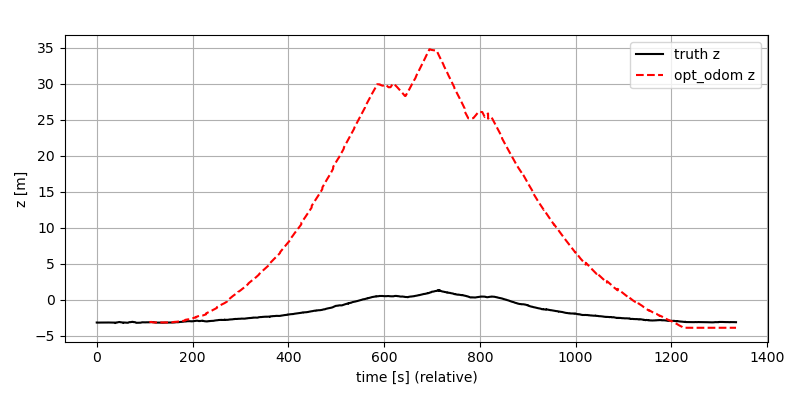
\includegraphics[width=\textwidth]{3-SLAM/3-results/figures/ds0_z.png}
        \caption{Baseline | Dataset 0}
    \end{subfigure}
    \hfill
    \begin{subfigure}[b]{0.48\textwidth}
        \centering
        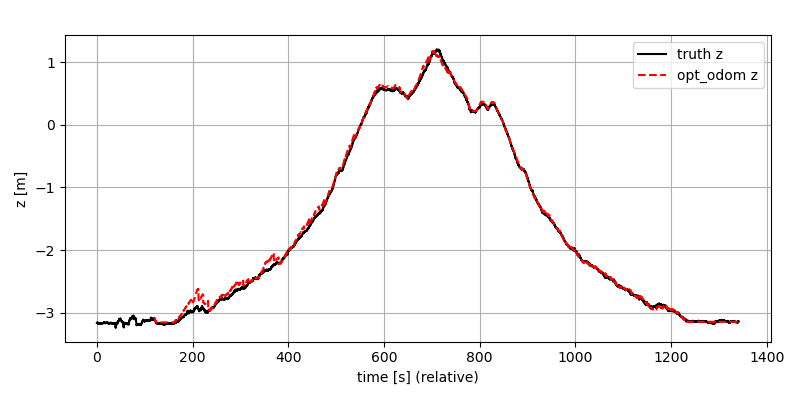
\includegraphics[width=\textwidth]{3-SLAM/3-results/figures/pds0_z.png}
        \caption{Proposed | Dataset 0}
    \end{subfigure}

    \vspace{1em} % Vertical space between rows

    % --- ROW 2 ---
    \begin{subfigure}[b]{0.48\textwidth}
        \centering
        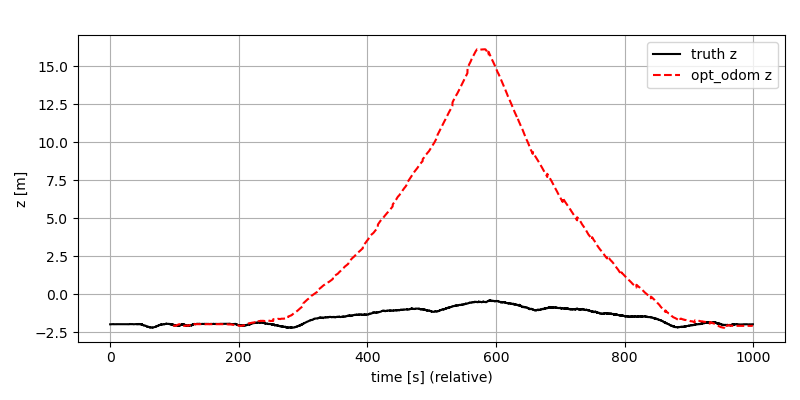
\includegraphics[width=\textwidth]{3-SLAM/3-results/figures/ds1_z.png}
        \caption{Baseline | Dataset 1}
    \end{subfigure}
    \hfill
    \begin{subfigure}[b]{0.48\textwidth}
        \centering
        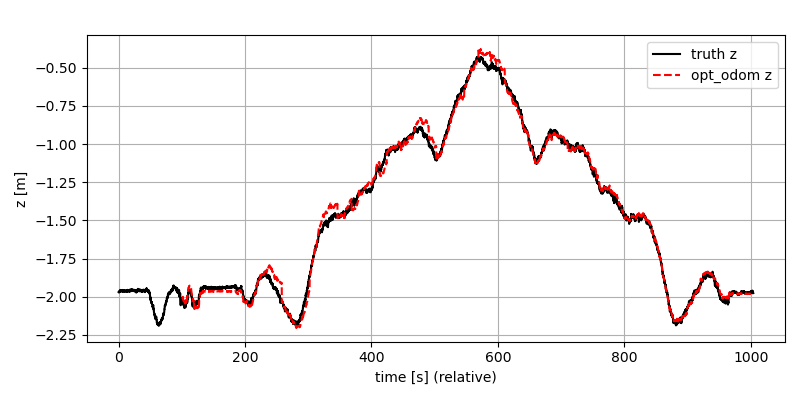
\includegraphics[width=\textwidth]{3-SLAM/3-results/figures/pds1_z.png}
        \caption{Proposed | Dataset 1}
    \end{subfigure}

    \vspace{1em}

    % --- ROW 3 ---
    \begin{subfigure}[b]{0.48\textwidth}
        \centering
        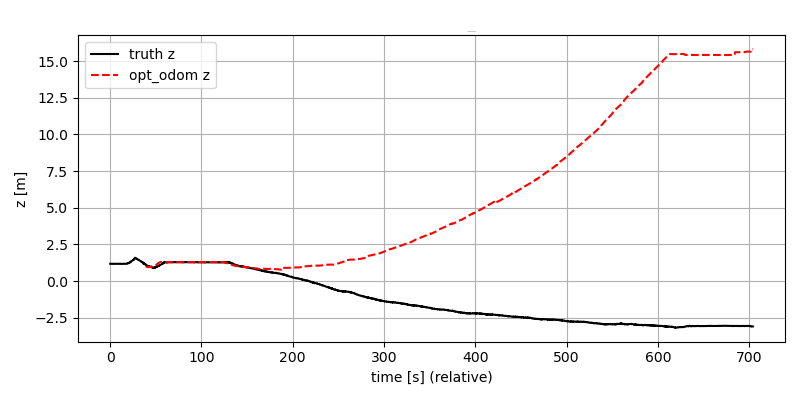
\includegraphics[width=\textwidth]{3-SLAM/3-results/figures/ds2_z.png}
        \caption{Baseline | Dataset 2}
    \end{subfigure}
    \hfill
    \begin{subfigure}[b]{0.48\textwidth}
        \centering
        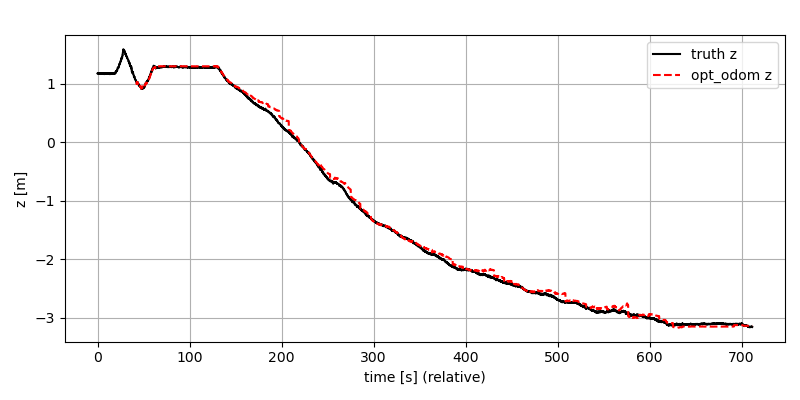
\includegraphics[width=\textwidth]{3-SLAM/3-results/figures/pds2_z.png}
        \caption{Proposed | Dataset 2}
    \end{subfigure}

    \vspace{1em}

    % --- ROW 4 ---
    \begin{subfigure}[b]{0.48\textwidth}
        \centering
        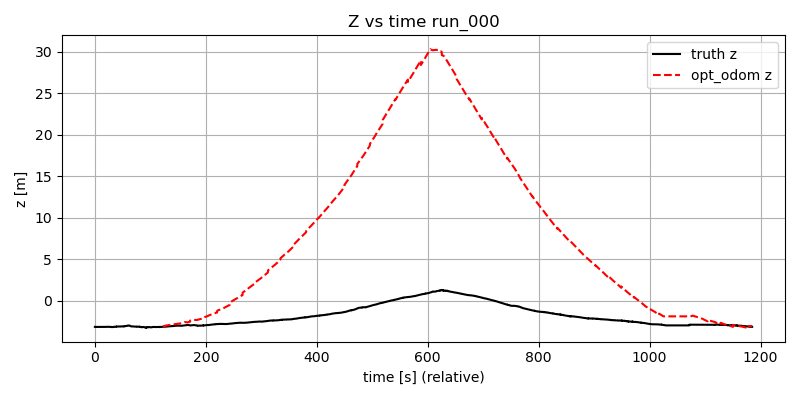
\includegraphics[width=\textwidth]{3-SLAM/3-results/figures/ds3_z.png}
        \caption{Baseline | Dataset 3}
    \end{subfigure}
    \hfill
    \begin{subfigure}[b]{0.48\textwidth}
        \centering
        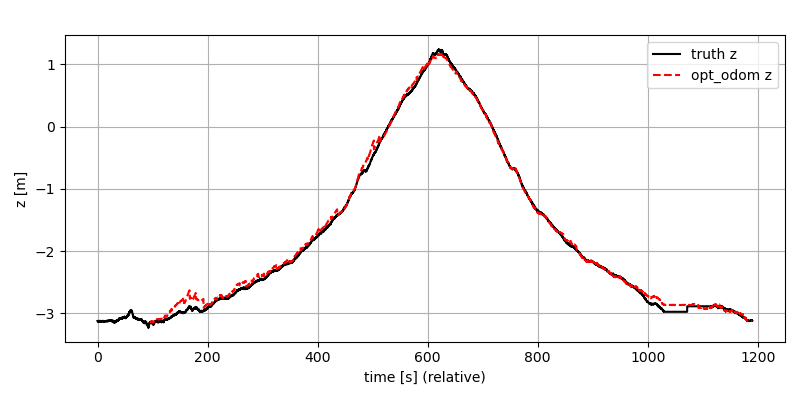
\includegraphics[width=\textwidth]{3-SLAM/3-results/figures/pds3_z.png}
        \caption{Proposed | Dataset 3}
    \end{subfigure}

    \vspace{1em}

    % --- ROW 5 ---
    \begin{subfigure}[b]{0.48\textwidth}
        \centering
        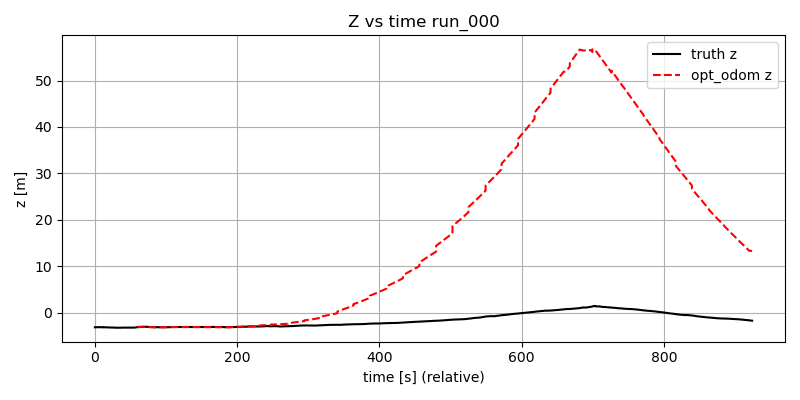
\includegraphics[width=\textwidth]{3-SLAM/3-results/figures/ds4_z.png}
        \caption{Baseline | Dataset 4}
    \end{subfigure}
    \hfill
    \begin{subfigure}[b]{0.48\textwidth}
        \centering
        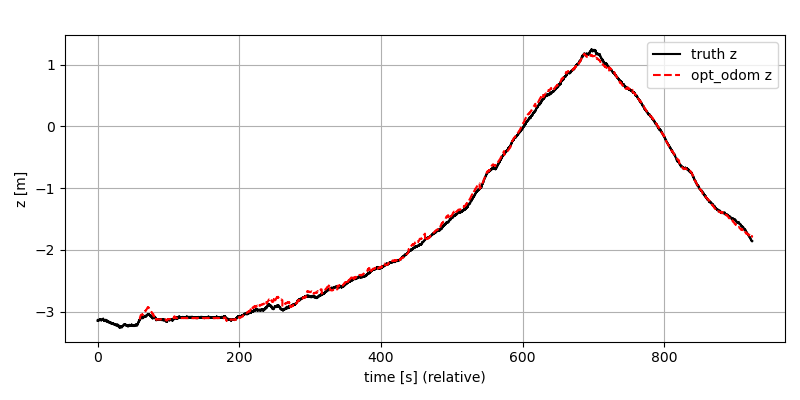
\includegraphics[width=\textwidth]{3-SLAM/3-results/figures/pds4_z.png}
        \caption{Proposed | Dataset 4}
    \end{subfigure}

    \caption{Trajectories in Z plane from baseline GLIM and the proposed method.}
    \label{fig:large_grid_z}
\end{figure}

\subsection{Evaluation Dataset Results}
\label{subsec:slam-eval-results}

The following subsections report performance on the held-out Evaluation Dataset as described in \cref{subsec:slam-experimental-setup}. Each configuration was evaluated across five independent runs; each table cell reports the aggregate statistic over those runs (mean, standard deviation, median, minimum, and maximum). This structure differs from the parameterisation dataset tables above, which report a single run per dataset.

\subsubsection{Baseline GLIM --- Evaluation Dataset}

\cref{tab:eval_baseline_performance} reports the baseline GLIM performance on the Evaluation Dataset. The mean error percentage per metre is 1.9612\% (std 0.4519\%), which falls within the range observed across the five parameterisation datasets (1.253\%--7.361\%). The mean RMSE 3D is 17.4799\,m and the mean ATE is 13.3863\,m, with the trajectory length averaging approximately 682\,m across the five runs.

\begin{table}[htbp]
\centering
\caption{Baseline GLIM performance on the Evaluation Dataset (mean, std, median, min, and max across five independent runs)}
\label{tab:eval_baseline_performance}
\begin{tabularx}{\textwidth}{lXXXXX}
\toprule
\textbf{Metrics} & \textbf{Mean} & \textbf{Std} & \textbf{Median} & \textbf{Min} & \textbf{Max} \\ \midrule
RMSE\ x\ (m)\        & 8.5597  & 5.6389 & 9.2456  & 2.1927  & 16.9319 \\
RMSE\ y\ (m)\        & 1.0545  & 0.5029 & 1.2180  & 0.2744  & 1.6128  \\
RMSE\ z\ (m)\        & 14.5590 & 2.2620 & 14.2411 & 11.9558 & 18.1913 \\
RMSE\ 3D\ (m)\       & 17.4799 & 3.6283 & 17.0259 & 12.2617 & 22.2915 \\
ATE\ (m)\            & 13.3863 & 3.1436 & 13.5756 & 9.1031  & 17.9034 \\
max\ error\ 3D\ (m)\ & 35.4544 & 6.6132 & 35.7962 & 24.9744 & 42.6418 \\
error\ per\ meter\ (m)\        & 0.0196  & 0.0045 & 0.0198  & 0.0134  & 0.0261  \\
error\ percent\ per\ meter\ (\%)\ & 1.9612  & 0.4519 & 1.9785  & 1.3390  & 2.6050  \\
RPE\ 1m\ translation\ RMSE\  & 0.1153 & 0.0649 & 0.1008 & 0.0466 & 0.2178 \\
RPE\ 1m\ translation\ mean\  & 0.0350 & 0.0080 & 0.0332 & 0.0253 & 0.0469 \\
RPE\ 1m\ translation\ std\   & 0.1093 & 0.0657 & 0.0952 & 0.0391 & 0.2127 \\
RPE\ 1m\ translation\ max\   & 1.6539 & 1.0152 & 1.4059 & 0.5472 & 3.2732 \\
RPE\ 10m\ translation\ RMSE\ & 0.1840 & 0.1104 & 0.1350 & 0.1202 & 0.3804 \\
RPE\ 10m\ translation\ mean\ & 0.0829 & 0.0354 & 0.0684 & 0.0640 & 0.1460 \\
RPE\ 10m\ translation\ std\  & 0.1638 & 0.1055 & 0.1163 & 0.1017 & 0.3513 \\
RPE\ 10m\ translation\ max\  & 1.8315 & 1.2155 & 1.3836 & 1.0030 & 3.9561 \\ \bottomrule
\end{tabularx}
\end{table}

\subsubsection{Refined GLIM --- Evaluation Dataset}

\cref{tab:eval_refined_performance} reports the refined GLIM performance on the Evaluation Dataset. The mean error percentage per metre is 0.6215\% (std 0.1089\%), consistent with the parameterisation dataset range of 0.608\%--3.615\%. However, the maximum 3D positional error exhibits a mean of 39.5938\,m with a standard deviation of 60.9811\,m and a maximum of 148.6057\,m, against a median of only 13.0861\,m. This large discrepancy between mean and median indicates that at least one run experienced a catastrophic failure, with the median providing a more representative estimate of typical performance. The same instability is evident in the RPE metrics, where the mean and standard deviation are far in excess of the corresponding median values.

\begin{table}[htbp]
\centering
\caption{Refined GLIM performance on the Evaluation Dataset (mean, std, median, min, and max across five independent runs). The high standard deviation on max error 3D, RPE 1\,m RMSE/std, and RPE 10\,m RMSE/std indicates that at least one run experienced a catastrophic localisation failure; median values are more representative of typical performance.}
\label{tab:eval_refined_performance}
\begin{tabularx}{\textwidth}{lXXXXX}
\toprule
\textbf{Metrics} & \textbf{Mean} & \textbf{Std} & \textbf{Median} & \textbf{Min} & \textbf{Max} \\ \midrule
RMSE\ x\ (m)\        & 5.5597  & 1.0624  & 5.6697  & 3.8536 & 6.7263   \\
RMSE\ y\ (m)\        & 1.6605  & 0.6931  & 1.3737  & 1.1688 & 2.8703   \\
RMSE\ z\ (m)\        & 0.8144  & 0.2925  & 0.8298  & 0.3895 & 1.2087   \\
RMSE\ 3D\ (m)\       & 5.8987  & 1.0561  & 6.2477  & 4.1607 & 6.9222   \\
ATE\ (m)\            & 4.3123  & 0.7479  & 4.4489  & 3.0535 & 4.9758   \\
max\ error\ 3D\ (m)\ & 39.5938 & 60.9811 & 13.0861 & 9.1552 & 148.6057 \\
error\ per\ meter\ (m)\        & 0.0062 & 0.0011 & 0.0065 & 0.0045 & 0.0072 \\
error\ percent\ per\ meter\ (\%)\ & 0.6215 & 0.1089 & 0.6501 & 0.4453 & 0.7192 \\
RPE\ 1m\ translation\ RMSE\  & 0.4082  & 0.8182  & 0.0443  & 0.0353 & 1.8718   \\
RPE\ 1m\ translation\ mean\  & 0.0301  & 0.0129  & 0.0249  & 0.0225 & 0.0531   \\
RPE\ 1m\ translation\ std\   & 0.4019  & 0.8213  & 0.0367  & 0.0272 & 1.8711   \\
RPE\ 1m\ translation\ max\   & 30.2296 & 66.2890 & 0.5803  & 0.5403 & 148.8110 \\
RPE\ 10m\ translation\ RMSE\ & 0.4625  & 0.8266  & 0.0864  & 0.0662 & 1.9405   \\
RPE\ 10m\ translation\ mean\ & 0.0591  & 0.0121  & 0.0534  & 0.0462 & 0.0766   \\
RPE\ 10m\ translation\ std\  & 0.4475  & 0.8342  & 0.0679  & 0.0474 & 1.9390   \\
RPE\ 10m\ translation\ max\  & 30.3526 & 66.1113 & 0.8106  & 0.5282 & 148.6158 \\ \bottomrule
\end{tabularx}
\end{table}

\subsubsection{Proposed Method --- Evaluation Dataset}

\cref{tab:eval_proposed_performance} reports the proposed method's performance on the Evaluation Dataset. The mean error percentage per metre is 0.0166\% with a standard deviation of 0.0004\%, indicating highly consistent performance across all five runs. The mean RMSE 3D is 0.1459\,m and the mean ATE is 0.1135\,m. The GASP metric has a mean of 0.0508 (std 0.0081), which is consistent with the range observed on the parameterisation datasets (0.0274--0.0679).

\begin{table}[htbp]
\centering
\caption{Proposed method performance on the Evaluation Dataset (mean, std, median, min, and max across five independent runs)}
\label{tab:eval_proposed_performance}
\begin{tabularx}{\textwidth}{lXXXXX}
\toprule
\textbf{Metrics} & \textbf{Mean} & \textbf{Std} & \textbf{Median} & \textbf{Min} & \textbf{Max} \\ \midrule
RMSE\ x\ (m)\        & 0.0958   & 0.0091   & 0.0949   & 0.0842   & 0.1070   \\
RMSE\ y\ (m)\        & 0.1010   & 0.0117   & 0.1067   & 0.0803   & 0.1074   \\
RMSE\ z\ (m)\        & 0.0426   & 0.0046   & 0.0433   & 0.0369   & 0.0493   \\
RMSE\ 3D\ (m)\       & 0.1459   & 0.0113   & 0.1493   & 0.1264   & 0.1535   \\
ATE\ (m)\            & 0.1135   & 0.0027   & 0.1131   & 0.1112   & 0.1179   \\
max\ error\ 3D\ (m)\ & 0.8573   & 0.1265   & 0.8569   & 0.6631   & 0.9732   \\
error\ per\ meter\ (m)\        & 0.000166 & 0.0000035& 0.000165 & 0.000163 & 0.000172 \\
error\ percent\ per\ meter\ (\%)\ & 0.0166   & 0.0004   & 0.0165   & 0.0163   & 0.0172   \\
GASP\                & 0.0508   & 0.0081   & 0.0520   & 0.0385   & 0.0607   \\
RPE\ 1m\ translation\ RMSE\  & 0.0526 & 0.0076 & 0.0542 & 0.0412 & 0.0620 \\
RPE\ 1m\ translation\ mean\  & 0.0284 & 0.0019 & 0.0287 & 0.0260 & 0.0307 \\
RPE\ 1m\ translation\ std\   & 0.0441 & 0.0080 & 0.0454 & 0.0319 & 0.0539 \\
RPE\ 1m\ translation\ max\   & 0.6703 & 0.1050 & 0.6443 & 0.5714 & 0.8132 \\
RPE\ 10m\ translation\ RMSE\ & 0.1120 & 0.0204 & 0.1048 & 0.0868 & 0.1355 \\
RPE\ 10m\ translation\ mean\ & 0.0729 & 0.0028 & 0.0739 & 0.0682 & 0.0755 \\
RPE\ 10m\ translation\ std\  & 0.0841 & 0.0251 & 0.0759 & 0.0536 & 0.1132 \\
RPE\ 10m\ translation\ max\  & 0.7674 & 0.2078 & 0.7978 & 0.5085 & 0.9709 \\ \bottomrule
\end{tabularx}
\end{table}

\subsubsection{Evaluation Dataset Comparative Summary}

\cref{tab:eval_comparison_key_metrics} presents a side-by-side comparison of the three methods on three key metrics across the Evaluation Dataset. The proposed method achieves the lowest mean value for all three metrics. The refined GLIM's mean RPE 1\,m translation standard deviation exceeds that of the baseline due to the contribution of the catastrophic failure run; the median values for this metric restore the expected baseline--refined--proposed ordering.

\begin{table}[htbp]
\centering
\caption{Comparison of key metrics on the Evaluation Dataset (mean, std, and median across five independent runs; best mean per row in bold)}
\label{tab:eval_comparison_key_metrics}
\begin{tabularx}{\textwidth}{>{\hsize=0.8\hsize}X >{\hsize=1.2\hsize}X X X X}
\toprule
\textbf{Metrics} & \textbf{Method} & \textbf{Mean} & \textbf{Std} & \textbf{Median} \\ \midrule

\multirow{3}{=}{error percent per meter (\%)}
 & Baseline GLIM  & 1.9612 & 0.4519 & 1.9785 \\
 & Refined GLIM   & 0.6215 & 0.1089 & 0.6501 \\
 & Proposed Method & \textbf{0.0166} & 0.0004 & 0.0165 \\ \midrule

\multirow{3}{=}{RPE 1m translation std}
 & Baseline GLIM  & 0.1093 & 0.0657 & 0.0952 \\
 & Refined GLIM   & 0.4019 & 0.8213 & 0.0367 \\
 & Proposed Method & \textbf{0.0441} & 0.0080 & 0.0454 \\ \midrule

\multirow{3}{=}{error per meter (m)}
 & Baseline GLIM  & 0.0196   & 0.0045    & 0.0198   \\
 & Refined GLIM   & 0.0062   & 0.0011    & 0.0065   \\
 & Proposed Method & \textbf{0.000166} & 0.0000035 & 0.000165 \\ \bottomrule

\end{tabularx}
\end{table}
